\documentclass[a4paper]{book}
\usepackage{extarrows}
\usepackage{amsmath,amsthm}
\usepackage{amsmath}
\usepackage{amssymb}
\usepackage{amsfonts}
\usepackage{answers}
\usepackage{eufrak}
\usepackage{eucal}
\usepackage{fancyhdr}
\usepackage{graphicx}
{\setlength\arraycolsep{2pt}
\usepackage{mathrsfs}
\usepackage{graphicx,fancyhdr}
\usepackage{graphicx} 
\graphicspath{ {./images/} }
\usepackage{caption}
\usepackage{CJKnumb}
\usepackage{titlesec}
\titleformat{\chapter}{}{}{0em}{\bf\huge}
\usepackage{amsthm}
\usepackage{cite}
\usepackage[utf8]{inputenc}
\usepackage[colorlinks,urlcolor=blue,citecolor=blue,linkcolor=blue]{hyperref}
\usepackage{tikz}
\usepackage{setspace}
\usepackage{xspace}
\usepackage{cite}
\usepackage{parskip}

\newtheorem{theorem}{Theorem}%[section]
\newtheorem{lemma}[theorem]{Lemma}%[section]
\newtheorem{example}{Example}%[section]
\newtheorem{remark}{Remark}%[section]
\newtheorem{note}{Note}%[section]
\newtheorem{proposition}{Proposition}%[section]
\newtheorem{definition}{Definition}%[section]
\newtheorem{conjecture}{Conjecture}%[section]
\newtheorem{corollary}{Corollary}%[section]
\newtheorem{problem}{Problem}%[section]
\newtheorem{condition}{Condition}%[section]

\renewcommand{\proofname}{\textbf{Proof}}

\newenvironment{ddd}{\begin{rmdef}\rm}{\end{rmdef}}                             
\newenvironment{eee}{\begin{rmexa}\rm}{\end{rmexa}}                             
\newenvironment{rrr}{\begin{rmrem}\rm}{\end{rmrem}}                                   
\newenvironment{pf}[1][Proof]{\par\noindent{\em #1}. }{\hfill\framebox(6,6)\par\medskip}

\usepackage{geometry}
 \usepackage[normalem]{ulem}
%\renewcommand{\baselinestretch}{1.5}

\geometry{left=2.5cm,right=2.5cm,top=2.5cm,bottom=2.5cm}

\newcommand{\Poincare}{Poincar\'e\xspace}
\newcommand{\Holder}{Hölder}

\usepackage{graphicx} %picture
\usepackage{float} %picture
\usepackage{subfigure} %picture

\usepackage[nottoc,notlot,notlof]{tocbibind}
%Hölder
%\renewcommand{\baselinestretch}{1.5}
\let\cleardoublepage\clearpage
\begin{document}

\begin{titlepage}\phantom{|}\vspace{0.75in}
\begin{center}
    \underline{THE ISOPERIMETRIC PROBLEM}
\end{center}
\begin{center}
    \underline{}
\end{center}
\vspace{1.5in}%{2.0in}
\begin{center}
    Dissertation submitted at the University of Leicester \\
    in partial fulfilment of the requirements for \\ 
    the degree of Bachelor of Science of Mathematics\\
\end{center}
\vspace{.5in}
\begin{center}
    by
\end{center}
\vspace{.5in}
\begin{center}
    Steven Cheung \\
    Department of Mathematics \\
    University of Leicester \\
\end{center}
\vspace{0.5in}
\begin{center}
    May 2024
\end{center}
\end{titlepage}

\tableofcontents
\thispagestyle{empty}
\chapter*{Declaration}                % The * means no number for this chapter
\pagenumbering{arabic}
\addcontentsline{toc}{chapter}{\hspace{0.2in}Declaration}
All sentences or passages quoted in this project dissertation from other
people's work have been specifically acknowledged by clear cross referencing
to author, work and page(s).  I understand that failure to do this amounts
to plagiarism and will be considered grounds for failure in this module and
the degree examination as a whole.


\bigskip

\noindent
Name: Steven Cheung


\bigskip

\noindent
Signed: (add the signature from adobe pdf editor)


\bigskip

\noindent
Date: 

%-------------------------------------------------------------------------------------
\chapter*{Abstract}
\addcontentsline{toc}{chapter}{\hspace{0.2in}Abstract}
In general, we want the maximum area whose boundary must pertain a specific length, this basic idea of the isoperimetric problem leaves many mathematicians puzzled still to this day.
\newline
\newline
\textbf{Rich History:} Our problem is one not to be trifled with, and across many a centuries to even dating back to 200 BC, we can see the events unfold of how we learn about how the small intricacies become part of something larger and more complex. 
\newline
\newline
\textbf{2-D Case:} The isoperimetric problem revolves around finding the shape that achieves the maximum enclosed area among all closed curves with a given length. Amongst the many simple curves, we identify that the circle is unique for pertaining the optimal area. We touch on Steiner's proof along the way to provide his insight into how this particular curve is maximal comparative to others. Additionally, show how the Euler-Lagrange Equation comes into effect; the finding of extremal curves with fixed areas and fixed perimeters. Our overall findings and conclusions are to show that across many a proofs through the decades, mathematicians have opted to find curves under this fixed perimeter constraint with additional factors taking place. Afterwards we focus on how Stokes' Theorem works with the inequality using a variety of calculus equations and figures in order to prove that the problem holds true under certain circumstances.
\newline
\newline
\textbf{3-D Case:} Most common example of the isoperimetric inequality seen in three dimensional space is through a water droplet. Spherical in nature which allows us to refer back to our 2-D case, but applying further mathematical skills we delve into the world of surfaces, tension and forces. Here we will discuss the spherical isoperimetric inequality. (Here we will add our findings and conclusions, along with further proofs: Topological, Calculus, ODE)
\newline
\newline
\textbf{N-Dimensions:} 
\newline
\newline
\textbf{Manifolds:} 
\newline
\newline
\textbf{Overview:} Follow along with us as we uncover historical insights, delve into mathematical expressions, and reveal connections between geometry, calculus, and many more fascinating fields of mathematics. This is the captivating story of understanding the isoperimetric problem.

%-------------------------------------------------------------------------------------
\chapter{Introduction}
%\addcontentsline{toc}{chapter}{\hspace{0.2in}Introduction}
\section{Historical Notes}
%\addcontentsline{toc}{section}{\hspace{0.2in}Historical Notes}
Isoperimeter, isos which is ancient Greek for equal and perimetron for perimeter. The isoperimetric perimetric problem, even though not properly formalized, was already thought about all throughout the history. 
\newline
\newline
Book V of Pappus of Alexandria's Mathematical collections ~\cite{wiegert2010sagacity} began with a preface titled ``On the Sagacity of Bees'', rather than the history of mathematicians past or their accomplishments to follow. This was written near the end of the 3rd century $A.D.$. Observing, Pappus credited the bees with ``a certain geometrical forethought'' (Thomas 593~\cite{ivor1941selections}) for their nearly faultless hexagonal comb structure. He wrote
\begin{center}
    \begin{quote}
        ``Bees know just this fact which is useful to them, that 
        the hexagon is greater than the square and the triangle 
        and will hold more honey for the same expenditure of 
        material in constructing each''
    \end{quote}
    (Thomas 593~\cite{ivor1941selections})
\end{center}
Beyond the efficiency of bees, Pappus prefaced, ``We'' he continued
\begin{center}
    \begin{quote}
        ``... will {}investigate a somewhat wider problem, namely that, 
        of all equilateral and equiangular plane figures having an equal 
        perimeter, that which has the greater number of angles is always great 
        and the greates of them all is the circle having it's perimeter equal to them''
    \end{quote}
    (Thomas 593~\cite{ivor1941selections})
\end{center}

Pappus then started working on the isoperimetric problem, which included numerous smaller problems within it. The main objective of the problem is to determine which of the planes and figures with the same perimeter has the largest area amongst them.

Although Pappus addressed the problem in the collections, it has been a topic of interest for centuries before. Appearing in both mathematical and literary materials and captivating the minds of mathematicians. 
\newline
\newline
The isoperimetric issue demonstrates ancient mathmaticians' perceptiveness and the consistency of mathematical endeavor over time, even in the modern age. The isoperimetric problem have been used by poets and historians, despite its mathematical nature. Most famously, Virgil made use of the concept in his Roman epic, The Aeneid. To quote Virgil
\begin{center}
    \begin{quote}
        ``At last they landed, where from far your eyes
        May view the turrets of new Carthage rise;
        There bought a space of ground, which Byrsa call'd,
        From the bull's hide they first inclos'd and wall'd.''
    \end{quote}
    (Book I of Aeneid~\cite{virgil1981aeneid})
\end{center}

Virgil's version has it that Dido, daughter of the king of Tyre, fled home after her brother killed her husband. Dido ended up on the north coast of Africa, where she bargained to buy as much land as she could enclose with an oxhide. Thus, she cut the hide into thin strips, presumably met and solved enclosing the largest area with a given perimeter - the isoperimetric problem. Dido may have been clever enough and chose an area by the coast to exploit the shore as part of the perimeter. But this mostly spoils the purity of posed problem. Kline concludes~\cite{kline1985mathematics}. The Aeneid was written between $29$ and $19 B.C.$.
\begin{figure}[h]
    \begin{center}   
        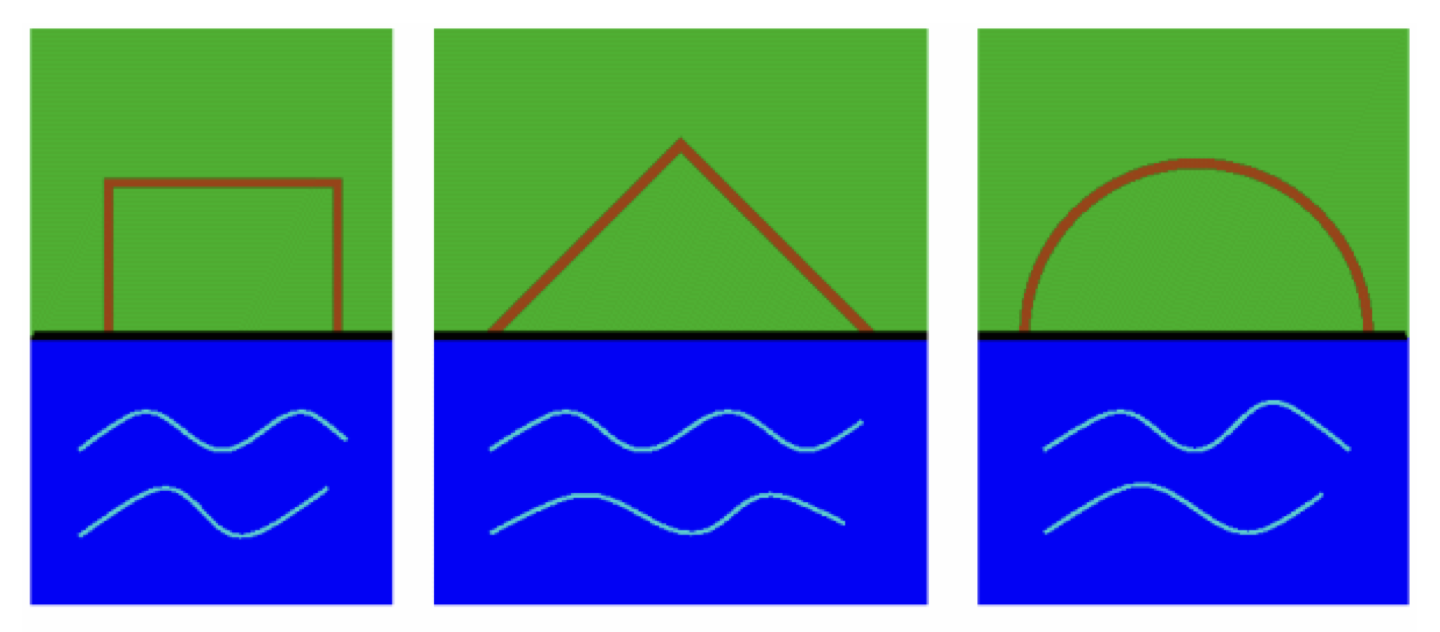
\includegraphics[width=120mm]{dido_1}
        \caption{Representations of areas bounded by common shapes of the same perimeter. The semicircle, answer to Dido's problem which contains the greatest area. (image and caption from~\cite{demjanenko2008isoperimetric})}
    \end{center}
\end{figure}
\leavevmode

In the 3rd century $A.D.$, Roman historian Marcus Junianus Justinus compliled an account of Carthaginian folklore that the legendary founding of Carthage by Dido, called Elissa by the Greeks (the mythological origin of the city):
\begin{center}
    \begin{quote}
        ``Then [Elissa] bout some land, just as much as could be covered by a cow's hide, where she could give some recreation to her men... She next gave orders for the hide to be cut into very fine strips, and in this way she took possession of a great area than she had apparently bargained for''
    \end{quote}
    (Book XVIII 157~\cite{yardley1994justin})
\end{center}

So since ancient Greece, around $100B.C.$, they wanted to measure the size of islands by timing how long it takes to circumnavigate the entire island. Proclus, a classical mathematician, mocked geometers for ``measuring the size of a city from the lengths of its walls''. To the common person of antiquity, two shapes with equal perimeter may have different areas. Interestingly, some individuals exploited this misconception to defraud others of land. Considerably more amusing, these con artists were viewed as liberal which demonstrates how unnatural the idea of shapes with a similar edge having different regions was to the old Greeks.
\newline
\newline
Geoffrey of Monmouth's Historia Regum Britanniae (History of the Kings of England), a 12th century $A.D.$ chronicle of Arthurian legends, mentions the isoperimetric problem. In this story, Hengist, a German duke, appeals to King Vortigern for land in exchange for his military service:
\begin{center}
    \begin{quote}
        ``'Grant', said Vortigern, 'unto thy servant but so much only as may be compassed round about by a single thong within the land thou hast given me, that so I ma build me a high place therein whereunto if need be I may betake me’...Straightaway...Hengist took a bull’s hide, and wrought the same into a single thong throughout. He then compassed round with his thong a stony place that he had right cunningly chosen, and within the space thus meted out did begin to build a castle that was afterwards called in British , Kaercorrei, but in Saxon, Thongceaster, the which in Latin’s speech is called Castrum corrigae'''
    \end{quote}
    (Monmouth 105-106~\cite{evans1920histories})
\end{center}
\leavevmode
\newline
\newline
Thus, the poets and historians who chronicled the exploits of these mythological characters as well as the figures themselves found special meaning in the isoperimetric problem. Despite its extensive implications, the notion of isoperimetry was ``naturally greek''. The Greeks have pretty much solved it, by their standards. Zenodorus was an ancient Greek mathematician from around $200B.C.$ to $120B.C.$. And have mostly proved that a circle has greater area than any polygon with the same perimeter. Majority of his work was lost. However, fortunately, parts of his work survived through references by Pappus and Theon of Alexandria.

Theon of Alexandria then develops this idea, with a summary of the proofs present by Zenodorus in ``On Isoperimetric Figures''. According to Theon, Zenodorus did not initiate his disussion of isoperimetry with the circle. Rather he stated that ``Of all rectilinear figures having an equal perimeter - I mean equilateral and equiangular figures - the greatest is that which has the most angles'' (Thomas 388-389~\cite{ivor1941selections}). In more modern language, the proposition is stated as follows: ``Given two regular $n$-gons with the same perimeter, one with $n=n_1$ and the other with $n=n_2>n_1$ then the regualr $n_2$-gon has the larger area'' (Nahin 47~\cite{nahin2021least}). Following this, Zenodorus was able to arrive at the proposition that "if a circle have an equal primter with an equilateral and equiangular rectilinear figure, the circle shall be the great" (Thomas 391~\cite{ivor1941selections}). As Heath notes in his ``History of Greek Mathematics'', Zenodorus chose to base his proof of this proposition on the theorem already established by Archimedes that ``the area of a circle is eaual to the right-angled triange with perpendicular side equal to the radius and base equal to the perimeter of the circle'' (Heath 209~\cite{heath2013history}). Frome here, Zenodorus proceeded on the basis of two preliminary lemmas: first that ``if there be two triangels on the same base and with the same perimeter one bein isosceles and the other scalene, the isosceles triangle has the greater area'' (Heath 209~\cite{heath2013history}); second that ``given two isosceles triangles not similar to one another, if [one constructs] on the same bases two triangles similar to one another such that the sme of the areas of the similar triangles is great than the sum of the ares of the non-similar triangles'' (Heath 210~\cite{heath2013history}). Both commentors seem to hint that it will be covered in subsequent chapters, but as Heath bemoans ``in the text as we have it the promise is not fulfilled'' (Heath 212~\cite{heath2013history}) (this entire paragraph is lifted from~\cite{wiegert2010sagacity})
\newline
\newline
In the ancient world, the problem of isoperimetry was associated with the work of Zenodorus and his commentator Pappus. It was the work of a  Swiss mathematician Jacob Steiner (1796-1863) who tackled the isoperimetric theorem in the modern word.

Indeed, the problem of isoperimetry in the niniteenth century emerged at an important juncture in mathematical thought. Mathematicians working in all fields of inquiry struggled over the use of analytic (i.e. calculus) or synthentic (i.e pure geometry) methods in solving problems.~\cite{wiegert2010sagacity} Nahin notes that Steiner's 1842 geometrical proof of the isoperimetric theorem is still regarded as a ``model of mathematical ingenuity'' despite subsequent discoveries of defects in the synthetic approach. The following propositions must be understood to be logically equivalent in order for Steiner's proof of the isoperimetric theorem to hold:
\begin{center}
    \begin{quote}
        A. ``Of all closed curves in a plane with equal perimeters, the cicle bounds the largest area''
        \newline
        [and]
        \newline
        B. ``Of all closed curves in a plane with equal areas, the cricle has the smallest perimeter''
    \end{quote}
    (Nahim 55~\cite{nahin2021least})
\end{center}

Steiner thought he had demonstrated that the circle was the answer to the isoperimetric problem. As later researchers, especially the German mathematician Peter Dirichlet (1805-1859), remarked, Steiner had made an underlying assumption not explicitly addressed in his proof, namely that a solution existed (Nahin 59~\cite{nahin2021least}).
\newline
\newline
Other mathematicians attempted to tackle the isoperimetric problem from the analytic or calculus-based perspective. And to no avail.

Problems posed by the ancients not only speeded the progression towards more rigorous, complete systems of mathematics, but also prompted later innovators to develop new systems to deal with these early questions. The isoperimetric problem thus demonstrates an important continuity in mathematical thought. From Zenodorus to Pappus and from Steiner to the mathematicians of the twenty-first century, isoperimetry has transcended its origins in ancient geometry to become a building block of more modern analytic systems of mathematics~\cite{wiegert2010sagacity}. Below is a table summary:
\begin{center}
    \begin{tabular}{||c c c||} 
        \hline
        Name & Time Period & What they did? \\ [0.5ex] 
        \hline
        Pappus & written 3rd Century $A.D.$ & started working about the isoperimetric problem \\ && from bee's hexagonal comb structure  \\ 
        \hline
        Dido (The Aeneid) & 29$B.C.$-19$B.C.$ & enclose as much land with oxhide \\
        \hline
        Zenodorus & 200$B.C.$-120$B.C.$ & more angles means more area \\
        \hline
        Ancient Greece & 100$B.C.$ & circumnavigate land \\
        \hline
        Arthurian Legends & 12th Century $A.D.$ & exchanged land for military service \\
        \hline
        Steiner & 1842 & first proof (existence) \\ 
        \hline
        Peter Dirichlet & 1805-1859 & noticed flaw with Steiner's proof \\ [1ex]
        \hline
    \end{tabular}
\end{center}

\section{Important Preliminaries}
%\addcontentsline{toc}{chapter}{\hspace{0.2in}Important Preliminaries}
We will take for granted the Jordan Curve Theorem
\begin{theorem}[Jordan Curve Theorem]
    A simple closed curve in the plane divides the plane into two regions, one compact and one non-compact, and in the common boundary of both regions.
\end{theorem}

The Jordan Curve Theorem is just a standard, but highly non-trivial, result of the topology of $\mathbb{R}^2$, that any simple closed curve in the plane has an 'interior' and 'exterior': more precisely, the complement of the image of $\gamma$ (i.e. the set of two points $\mathbb{R}^2$ that are \underline{not} in the image of $\gamma$) is the disjoint union of two subsets of $\mathbb{R}^2$, denoted by $int(\gamma)$ and $ext(\gamma)$, with the following properties:
\begin{enumerate}
    \item $int(\gamma)$ is bounded, i.e. it is contained inside the circle of sufficiently large radius.
    \item $ext(\gamma)$ is unbounded
    \item Both of the regions $int(\gamma)$ and $ext(\gamma)$ are connected, i.e. they have the property that any two points in the same region can be joined by a curve contained entirely in the region (but any curve joining a point of $int(\gamma)$) to a point of $ext(\gamma)$ must cross the curve $\gamma$)
\end{enumerate}


\begin{note} 
    When we talk of the region bounded by a simple closed curve in the plane, we always mean the compact region
\end{note}

\begin{definition}
    A closed curve, is a curve that changes direction but does not cross itself whilst changing direction.
\end{definition}

\begin{definition}
    A simple curve, is a curve that changes direction but does not cross itself whilst changing direction.
\end{definition}

\begin{definition}
    A simple closed curve in $\mathbb{R}^2$, is a closed curve in $\mathbb{R}^2$ that has no self-intersections
\end{definition}

The two definitions, above, are vital into understanding the main theorem. Since the isoperimetric inequality is a global result, we borrow concepts from topology, such as:

\begin{definition}
    A function is bounded if $\exists M \in \mathbb{R}$ such that $\left| f(x) \right| \leq M$.
\end{definition}

\begin{definition}
	Let $f:D\to\mathbb{R}$ a function and $c\in\mathbb{R}$ such that there exists $p>0$ such that $(c-p,c+p)\in D$. Then $f$ is called \textit{continuous} at $c$ if
	\begin{center}
		$\underset{x\to c}{\lim}f(x)=f(c)$.
	\end{center}
\end{definition}

\begin{definition}
    Let $X$ be a topological space and $A \subset X$. An open cover for $A$ is a family $\{U_\lambda\}_{\lambda\in I}$ of open subsets of $X$ such that
    \begin{center}
        $A \subset\underset{\lambda\in I}{\bigcup}{U_\lambda}$
    \end{center}
    An open cover is called finite if $\|I\|<\infty$. If $\{U_\lambda\}_{\lambda\in I}$ is an open cover for $A$ and $J \subset I$ is such that $A\subset\underset{\lambda\in J}{\bigcup}{U_\lambda}$, then $\{U_\lambda\}_{\lambda\in J}$ is called a subcover of $\{U_\lambda\}_{\lambda\in I}$.
\end{definition}

\begin{definition}
    A subset $A \subset X$ of a topological space called compact if every open cover of $A$ has a finite subcover. A space is called compact space if it is a compact subset of itself.
\end{definition}

\begin{definition} (Heine-Borel Theorem)
    A set in $\mathbb{R}^n$ is said to be compact if it is closed and bounded.
\end{definition}

\newpage
\subsection{Basics in Convex Geometry}
You may be wondering why we would study convex geometry but this is the necessary language and notation, which will be used in the following sections. Convex geometry will give us a way to describe objects and sets in Euclidean space; We consider convex, compact sets in $\mathbb{R}^n$ and their properties (areas, volumes, etc). The term convex is used to refere to a shape that has a curve or a protuding suface. In other words, all the lines across the outline are straight and they point outwards. Examples of convex polygons are signboard, a football, etc. The complement of convex is concave, where the shape curves inwards and no protuding surface at some point. For example the inside of a bowl. A clear definition of when a set is convex is given below. 

As our goal is to maximize, get the largest area, it is quite clear on why we choose convex curves over concave curves. When studying the polygons, it is easy to think that all convex polygons are regular as all regular polygons are convex, but that is not the case.
\newline

\begin{definition}
	A set $A\subseteq\mathbb{R}^n$ is called $convex$ if all $x,y\in A$ satisfy $(1-\lambda)x+\lambda y\in A$, $\forall\lambda\in[0,1]$.
\end{definition}

\begin{remark}
	Intersections of convex sets, and for affine maps the pre-image and the image of convex sets are also convex. Let $A, B \subset\mathbb{R}^n$ be convex and $\lambda\in\mathbb{R}$. Then
	\begin{center}
		$\lambda B=\{x\in\mathbb{R}^n;\exists b\in B$ with $x=\lambda\dot b\}$, and
	
		$\lambda+B=\{x\in\mathbb{R}^n;\exists a\in A, b\in B$ with $x=a+b\}$
	\end{center}
	are also convex
\end{remark}

\begin{definition}
	Let $A\subseteq\mathbb{R}^n$ be non-empty, compact and convex. Then $A$ is called $convex$ $body$. The set of all convex bodies of $\mathbb{R}^n$ is denoted by $\mathscr{K}^n$ and the set of all convex bodies in $\mathbb{R}^n$ with non-empty interior is denoted by $\mathscr{K}_{0}^{n}$.
\end{definition}

\begin{definition}
	\begin{itemize}
		\item Define $\bar{R}=\mathbb{R}\cup\{ \infty,-\infty\}$.
		\item A function $f:\mathbb{R}^n\to\bar{\mathbb{R}}$ is called $proper$ if it satisfies $\{f=-\infty\}=\emptyset$ and $\{f=\infty\}\neq\mathbb{R}^n$.
		\item A proper function $f:\mathbb{R}^n\to\bar{\mathbb{R}}$ is called $convex$ if it satisfies 
		\begin{center}
			$f((1-\lambda)x+\lambda y)\leq(1-\lambda)f(x)+\lambda f(y)$
		\end{center}
		for all $x, y\in\mathbb{R}^n$ and $0\leq\lambda\leq1$.
		\item . A function $f:D\to\bar{\mathbb{R}}$ with $D\subseteq\mathbb{R}^n$ is called convex if its expansion on $\mathbb{R}^n$
		\begin{center}
			\begin{equation}
				  \tilde{f}(x):=\begin{cases}
				    	f(x), & \text{for $x\in D$}.\\
				   	 \infty, & \text{otherwise}.
				  \end{cases}
			\end{equation}
		\end{center}
		is convex.
		\item A function $f$ is $concave$ if $-f$ is convex.
	\end{itemize}
\end{definition}
(Some Figure here)
%-------------------------------------------------------------------------------------

\chapter{2-Dimensional Case ($\mathbb{R}^2$)}
\begin{theorem}
    Let $C$ be a simple closed curve in the plane with length $L$ and bounding a region of area $A$ . 
    Then $L^2 \leq 4\pi A$ with equality if and only if $C$ is a circle.
\end{theorem}
The circle therefore bounds the biggest area among all simple closed curves in the plane with a given length.

\section{Seven Proofs Concerning Variants of the Isoperimetric Property}
This is possibly may be one of the oldest problem in differential geometry. With that it comes with multiple mathematicians trying to prove the problem and or simplify the problem. The first considered real and rigorous proof was by Jakob Steiner however it had an apparent flaw, later indicated by K. Weierstrass. That it only proved the existence. In fact the isoperimetric problem was only a corollary of a theory developed by Weierstrass to handle problems of maximizing or minimizing certain integrals, this theory is called calculus of variations. More direct proofs were discovered later. We will mainly look at J.Steiner's and E.Schmidt's proof but the other proofs are mainly here to give additional insight on how to think about this problem. 

The seven proofs were done by Jakob Steiner, Karl Weierstrass, Erhard Schmidt, Vladimir Boltjanski, Richard Demar, Alfred D. Garvin, David Singmaster and D.J.Souppouris, and Gary Lawlor. This section is mostly studied from Kimberly Holman as her Masters Thesis~\cite{holman2022isoperimetric}.

\subsection{Jakob Steiner}
Firstly, we will look at this proposition. Isosceles triangle has the smallest leg-sum compared to trianges of the same baselien and either height or area, and vice-versa. Given an uneqal triangle, we want to maximise area on a triangle with the same baseline. We make the other two sides, not the baseline, equal. The result is a triangle witha smaller leg-sum, and therefor a smaller perimeter, containigng the same area. Now we can expand on the previous principle to demonstrate that any parallel trapezoid with unequal angles on one baseline may be transformed into another of the same area and baselines; Moreover, the new parallel trapezoid will have symmetry along the axis formed by the baseline midpoints and a smalelr sum of side lengths.

\subsection{Karl Weierstrass}
Relying on calculus of variation, this proof defines area and length in terms of integrals. However Karl Weierstrass's calculus of variation is very strong, and that the isoperimetric problem pops out of it. Calculus of variations is concerned with the problem of extremising "functionals", finding extrema of functions of \textit{infinite} variables. Functionals can be looked at like "functions of functions". The result is two Euler-Lagrange equations which when solved, provide an equation in the form of a circle and the length of the radius which optimizes the area given the length of the perimeter. The lagrangian, denoted by $L(x,y,y')$ normally opted as $L=T-V$, the kinetic energy minus the potential energy. Extremal curves represent solutions to the isoperimetric problem, providing the shapes that maximize the enclosed area under a fixed perimeter. Extremal curves are smooth and regular, ensuring the validity of the Euler-Lagrange equation and the associated boundary conditions. We shall not give proofs to these theorem and lemmas.
\begin{theorem}
	Consider the functional $J(Y)$, an extremum, defined as follows:
	\begin{center}
		$J[y]=\int_{a}^{b}L(x,y,y')\,dx$
	\end{center}
	where $L(x,y,y')$ is the lagrangian and $y'$ denotes the derivative of $y$ with respect to $x$. The critical points of $J[y]$ satisfy the Euler-Lagrange equation:
	\begin{center}
		$\frac{\partial}{\partial x}(\frac{\partial L}{\partial y'})-\frac{\partial L}{\partial y}=0$
	\end{center}
\end{theorem}
\begin{remark}
	$Y$ satisfying the Euler-Lagrange equation is a necessary, but not sufficient, condition for $J(Y)$ to be an extremum. In other words, a function $Y(x)$ may satisfy the Euler-Lagrange equation even when $J(Y)$ is not an extremum.
\end{remark}
\subsubsection{Isoperimetric with Lagrangian}
For the isoperimetric problem, the Lagrangian $L(x, y, y')$ becomes the integrand of the perimeter functional, which is the square root of $1 + (y')^2$.
\begin{center}
	$L(x, y, y') = \sqrt{1 + (y')^2}$
\end{center}
Applying the Euler-Lagrange equation to this Lagrangian, we get:
\begin{center}
	$\frac{d}{dx} \left( \frac{y'}{\sqrt{1 + (y')^2}} \right) - \frac{y}{\sqrt{1 + (y')^2}} = 0$
\end{center}
\begin{lemma}(\textbf{Existence of Extremal Curves})
        There exists at least one extremal curve that satisfies the Euler-Lagrange equation and corresponds to a critical point of the functional \( J[y] \).
    \end{lemma}

    \begin{lemma}(\textbf{Uniqueness of Extremal Curves})
        Under certain regularity conditions, there exists a unique extremal curve that satisfies the Euler-Lagrange equation and optimizes the area under a fixed perimeter.

        Solving the differential equation subject to the fixed endpoints~\cite{goldstein1980classical} and~\cite{hilbert1985methods}, along with the fixed area constraint, leads us to the discovery of extremal curves that not only minimize the perimeter but also provide profound insights into the Isoperimetric Inequality in two-dimensional spaces.
    \end{lemma}
Direct proofs from Weierstrass' corollary can be found in $Curves$ $and$ $Surfaces$ $in$ $Euclidean$ $Spaces$~\cite{chern1966curves}.

\subsection{Erhard Schmidt}
E.Schmidt simplified the work of Weierstrass to whom provided a complete proof of the Isoperimetric problem, however this proof seemed difficult to digest thus later mathematicians came in to assist, decades later. Beginning with parameterised curves, a circle is defined using carefully selected intervals and bounding. Using advanced calculus, isoperimetric equality is obtained if all calculated isoperimetric inequality statements are equalities. But here we will start off with the initial formula that we will see down below and how this initial formula will be used.

\textbf{Initial Formula}
Area, A, bounded by a positively oriented simple closed curve where: 
\begin{center}
	$\alpha(t)=(x(t),y(t)), t\in [a,b]$
\end{center}
\begin{center}
	$A=-\int_{a}^{b}y(t)x'(t)\,dt=\int_{a}^{b}x(t)y'(t)\,dt = 1/2\int_{a}^{b}(xy'-yx')\,dt$
\end{center}

\subsection{Vladimir Boltjanski}
Boltjanski's work provided a summary of Steiner's isoperimetric proof. Which starts off by showing that the maximum area of the shape must be convex.
\begin{proof}
	\begin{enumerate}
		\item Towards a general shape. He makes a "cross-cut" that divides the boundary into two equal lengths. If every cross-cut has equal area then the shape is extremal. Otherwise, omit the side with smaller area and reflect the larger area across the cross-cut. We may continue in this way until every cross-cut. We may continue in this way until every cross-cut has equal area.
		\item Now  he takes a fixed cross-cut, $a$, $b$, and any boundary points distinct from $a$ and $b$, $c$, and demonstrates that the extremal must have $\angle acb=90^{\circ}$. If the angle is anything else, install a hinge and rotate about $c$ until the angle mesaure of $acb$ is $90^{\circ}$.
		\item The reflect over the cross-cut to achieve a shape with greater area and same perimeter.
	\end{enumerate}
\end{proof}

\subsection{Richard Demar}
Demar begins with an indirect proof to show that the extremal is convex, then proceeds with a trivial example that the square is not extremal. While the square example is trivial and can easily be proved computationally, the trick Demar uses here will be used in subsequent proofs.

\subsection{Alfred D. Garvin}
Expanding on the work of Demar, physical experiments are performed to prove the statements. First, liquid mercury is slowly poured into a confined triangular reservoir and is expected to take on an isoperimetrically optimal configuration, which it does. However, the meniscus effect of the mercury slightly skews the endpoints of the arcs. Next, the reservoir is partially filled with water. A viscous oil is poured slowly onto the water and is expected to take on an isoperimetrically optimal shape, which it does. Again, the meniscus effect of the oil slightly skews the endpoits of the arcs. The third experiment uses a flexible, asymmetrical triangular wood fence and a sturdypaper closed fence with perimeter less than that of the triangle. BB pellets are poured inside the paper fence, which is expected to take on an isoperimetrically optimal shape, which it does. This internal-pressure experiment does not yield any skewed results. The three experiments yield the same description of the isoperimetrically optimal shape: the arcs have equal radii, the arcs have equal chords, and the arcs have equal length.

\subsection{David Singmaster and D.J. Souppouris}
The ratio of area to perimeter, A/P, is examined to find the set which produces the greatest number. Using advanced calculus and analysis, the maximal ratio of A/P is a measure of the circularity of the set.

\subsection{Gary Lawlor}
A new proof of the planar isoperimetric property is presented. The method is a slicing and covering argument, and calls for strategically dividing the circle as well as another, arbitrary region of equal perimeter, into tiny pieces. Each pieces from non-circle region contains the same length of the region’s boundary and has less area than the piece of the circle containing the same length of the circle’s boundary. An advantage of this proof is, as it is comparative, it does not require a proof of existence of an optimum solution.

\begin{lemma} 
    Among all the triangles with the same base, the isosceles triangle covers the greatest area.
\end{lemma}
\begin{figure}[h]
	\centering
	\begin{minipage}{0.5\textwidth}
		\centering
        		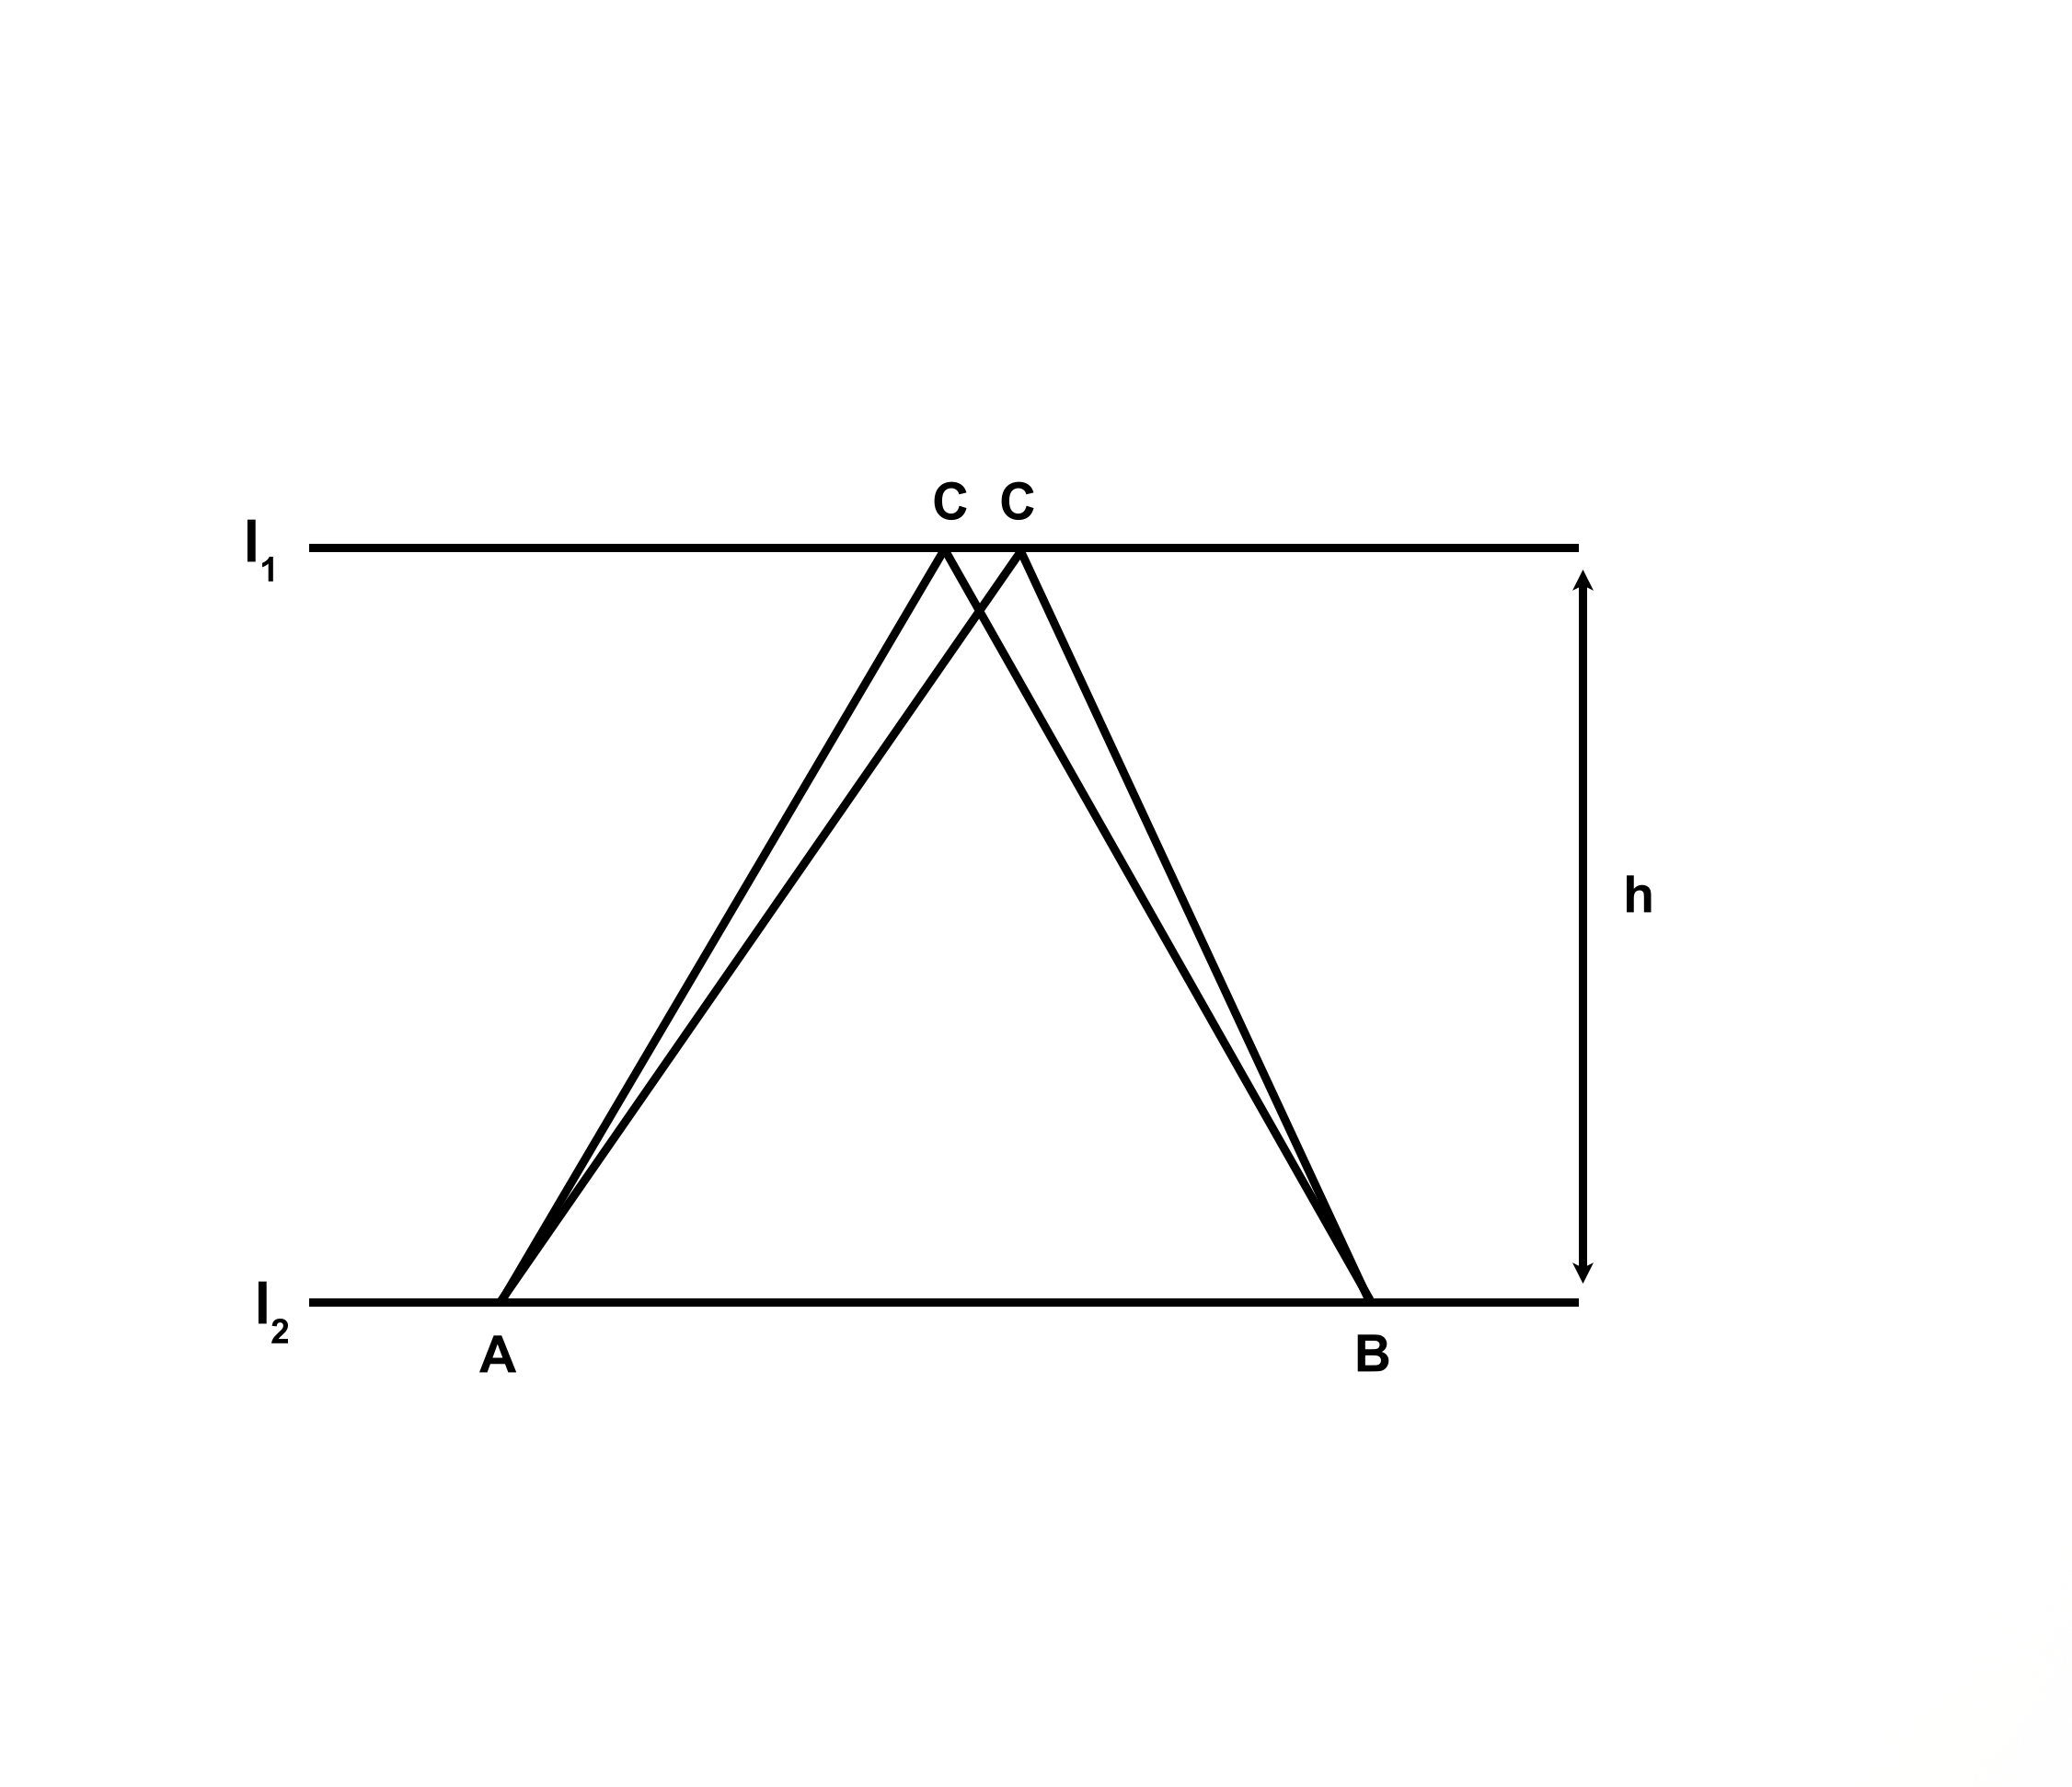
\includegraphics[width=65mm]{isofig5.png} % first figure itself
        		\caption{Figure I}
		%Tikz
		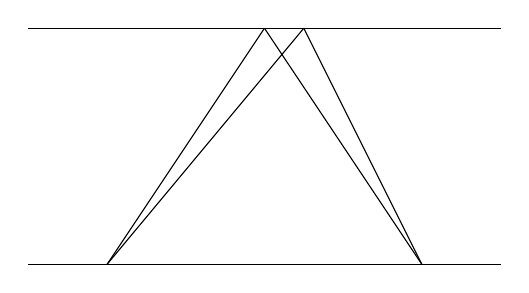
\begin{tikzpicture}
			%\pgfdeclarelayer{nodelayer} 
			%\pgfdeclarelayer{edgelayer}
			%\pgfsetlayers{main,nodelayer,edgelayer}
			% nodes
			%\begin{pgfonlayer}{nodelayer}
			%	\node [style=none] (A) at (0,10) {};
			%	\node [style=none] (B) at (6,10) {};
			%	\node [style=none] (C) at (0,13) {};
			%	\node [style=none] (D) at (6,13) {};
			%\end{pgfonlayer}
			% horizontal parallel lines
			%\begin{pgfonlayer}{edgelayer}
				\draw (0,10) -- (6,10);
				\draw (0,13) -- (6,13);
				% diagonal lines
				\draw (1,10) -- (3,13);
				\draw (3,13) -- (5,10);
				\draw (1,10) -- (3.5,13);
				\draw (3.5,13) -- (5,10);
			%\end{pgfonlayer}{edgelayer}
		\end{tikzpicture}
	\end{minipage}\hfill
    	\begin{minipage}{0.5\textwidth}
		\centering
		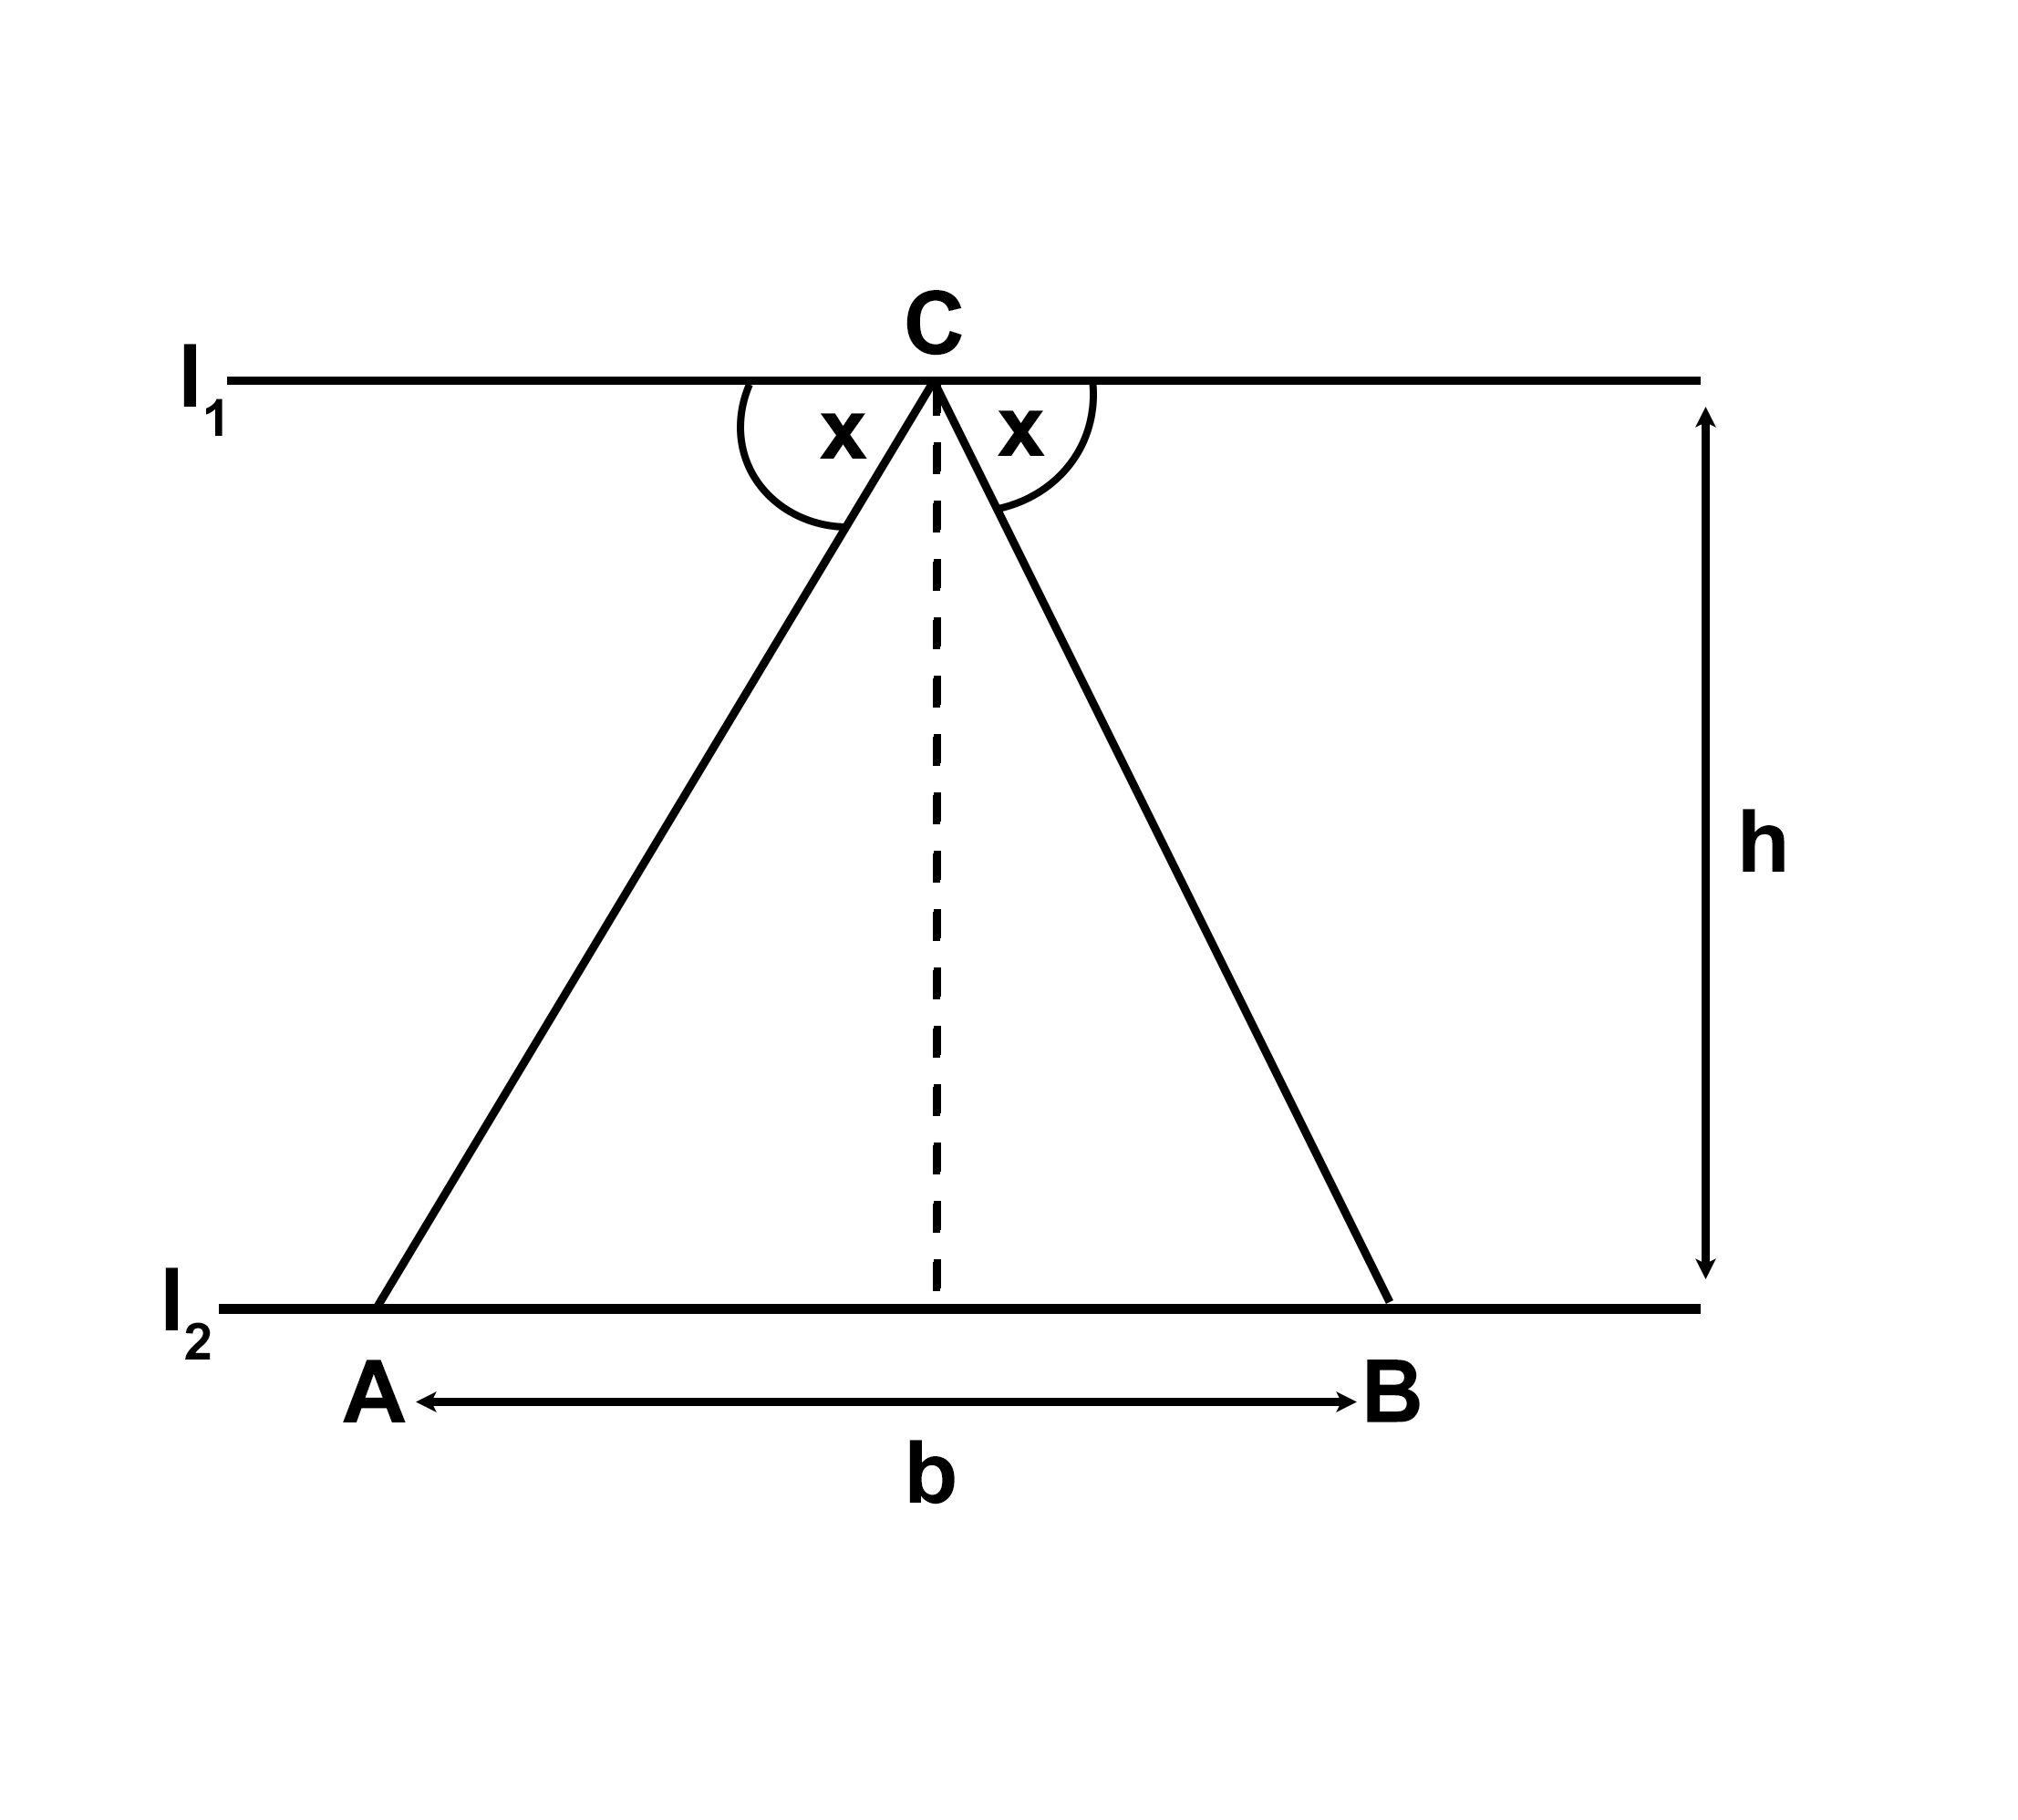
\includegraphics[width=65mm]{isofig6.png} % second figure itself
		\caption{figure II}
	\end{minipage}
\end{figure}
\begin{proof} 
    Let us consider the triangle ABC with base AB=b, looking at the figure above then our statement is logically equivalent to minimising AC+CB, since the area is just the product of the base and the height, we can slide C along the line $l_1$ this will preserve the area but alter the length of AC+CB, now to prove that the triangle shown in figure II minimises AC+CB we will use some inpiration from physics, lets consider a ray of light travelling from A to the line L, reflecting and then travelling back to B, now from the laws of attraction, light takes the shortest path, and the laws of reflection tells us that the angle of incident is equal to the angle of reflection with respect to the normal, in other words, for our scenario this means that AC=CB since the angles are the same. 
\end{proof}

\begin{lemma}
    For a given perimeter the equilateral triangle has the biggest area of all the triangles. 
\end{lemma}
\begin{proof} 
    Well from our previous diagram we can treat AC as the base and follow the same logic to arrive at the conclusion that CB=AB, similarly, treat CB as the base and follow the exact steps to arrive at the conclusion AC=AB, so from all of this we can conclude that AB=BC=AC, and so the equilateral triangle maximises the area.
\end{proof}

\begin{theorem}
    Among regular polygons with fixed perimeter, an increase in the number of sides results in a larger area.    
\end{theorem} 

\begin{minipage}{\linewidth}
    \centering
    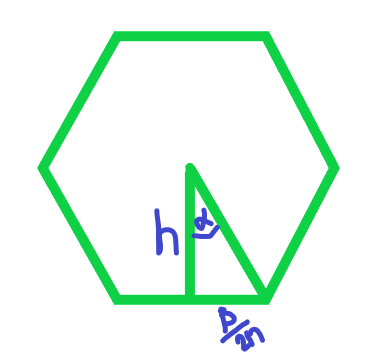
\includegraphics[width=7cm]{isofig10.png}
    \captionof{figure}{Figure III}
\end{minipage}
\begin{proof} 
    Let $P$ be the perimeter of of this n sided polygon In addition let $h$ be the apothem, which is the perpendicular which goes from the centre to a side. Then the area of the polygon is A where,  $A=\frac{1}{2} hP$. By considering the diagram above we can see that as n increases the length of the sides as well as the angle $\alpha$ decreases which means h increases. Well this means that the area must increase as $P$ is fixed and $h$ is increasing.
\end{proof}
\begin{theorem}
	If L is the perimeter and A is the area of any regular 2n-sided polygon, then 
	\begin{center}
		$L^{2}\geq8n*A*\tan{(\frac{\pi}{2n})}$
	\end{center}
\end{theorem}

\begin{figure} [h]
    \centering
    \begin{minipage}{0.5\textwidth}
        \centering
        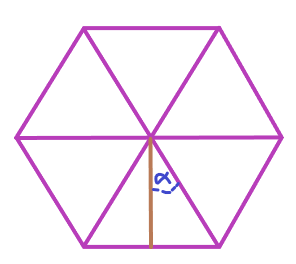
\includegraphics[width=1\textwidth]{isofig8.png} % first figure itself
        \caption{Figure V}
    \end{minipage}\hfill
    \begin{minipage}{0.5\textwidth}
        \centering
        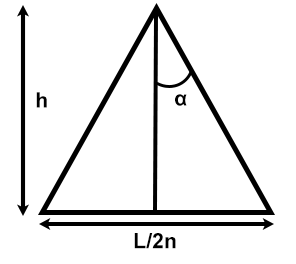
\includegraphics[width=1\textwidth]{isofig9.png} % second figure itself
        \caption{figure VI}
    \end{minipage}
\end{figure}

\begin{proof}
    	Since its a regular polygon we could consider one of the 2n triangles its made off as shown in the figure above. 
	\begin{center}
		$\displaystyle \tan(\alpha)=\frac{(\frac{L}{4n})}{h}$
	\end{center}
    	Rearranging the formula to make h the subject as well as using the fact that $\alpha=\frac{2\pi}{2n} \frac{1}{2}=\frac{\pi}{2n}$, we get 
	\begin{center}
		$\displaystyle h=\frac{L}{4n} \frac{1}{\tan(\frac{\pi}{2n})}$
	\end{center}
	Now for the area of the above triangle we get $\frac{1}{2}h*\frac{L}{2n}$
    	Substituting h, we obtain
	\begin{center}
		$\displaystyle \frac{L^{2}}{16n^{2}} \frac{1}{\tan(\frac{\pi}{2n})}$
	\end{center}
    	Finally, we consider the area of the whole polygon which is just 2n times of the above expression. So we have 
	\begin{center}
    		$\displaystyle A=\frac{L^{2}}{8n} \frac{1}{\tan(\frac{\pi}{2n})}$
	\end{center}
    	Since this is the optimal area we can be more precise and by rearranging the express we can conclude our desired expression which was $L^{2} \ge 8nA\tan(\frac{\pi}{2n})$
\end{proof}

\section{Unpacking J.Steiner's proof}
The proof that I will be unpacking and taking a closer look at will be from the book (reference the book here), and is credited by them to Jakob Sternier. Packed and concise proof from~\cite{gluck2012isoperimetric}. To reiterate, the German mathematician Peter Dirichlet (1805- 1859), remarked, Steiner had made an underlying assumption not explicitly addressed in his proof, namely that a solution existed (Nahin 59~\cite{nahin2021least}). A rather helpful computer visualisation, before we start the proof, to aid in the identification that indeed the circle is an answer, and how naturally a compressed circle (ellipse) has less area than a full and complete circle.
\begin{minipage}{\linewidth}
    \centering
    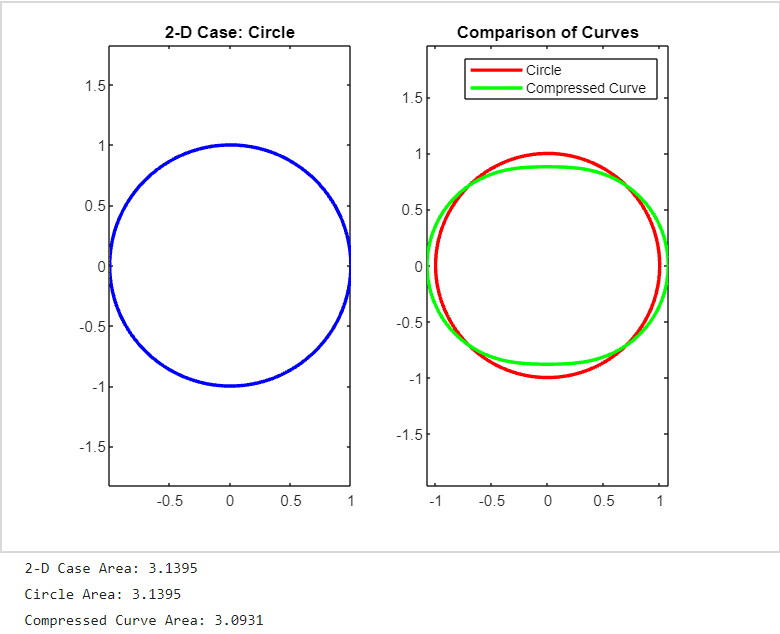
\includegraphics[width=150mm]{steinerproofvisualisation.png}
    \captionof{figure}{Area comparison of curves, Steiner's Proof}
\end{minipage}
\begin{proof}
    We will begin the proof by assuming the existence of a solution. In other words, that there exists a simple closed curve C of a specified length L, enclosing a region with the maximum possible area.
    \begin{enumerate}
        \item We claim that the curve C must by convex, meaning that any straight line connecting two points (O and A) on C should entirely lie within the region enclosed by C. We justify this assertion thus, suppose that the curve is not convex then we could draw a segment OA connecting the two points of C, with the entire segment (except for its endpoints) situated outside of C. By mirroring the relevant arc of C between O and A along this line, a new curve of an identical length emerges, encapsulating a greater area, as illustrated in the figure below. Therefore, C is already a convex curve.

        \begin{minipage}{\linewidth}
            \centering
            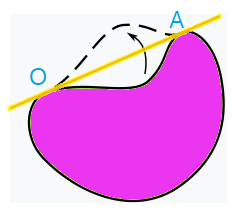
\includegraphics[width=70mm]{isofig1.png}
            \captionof{figure}{Figure VII}
        \end{minipage}
        \item Select two points, P and Q, to partition our solution curve C into arcs of identical length. Consequently, the line segment PQ must divide the region enclosed by C into two sections of equal area. Failure to do so would imply that the portion with a larger area could be mirrored across PQ, resulting in another curve of the same length but with greater area.

        \begin{minipage}{\linewidth}
            \centering
            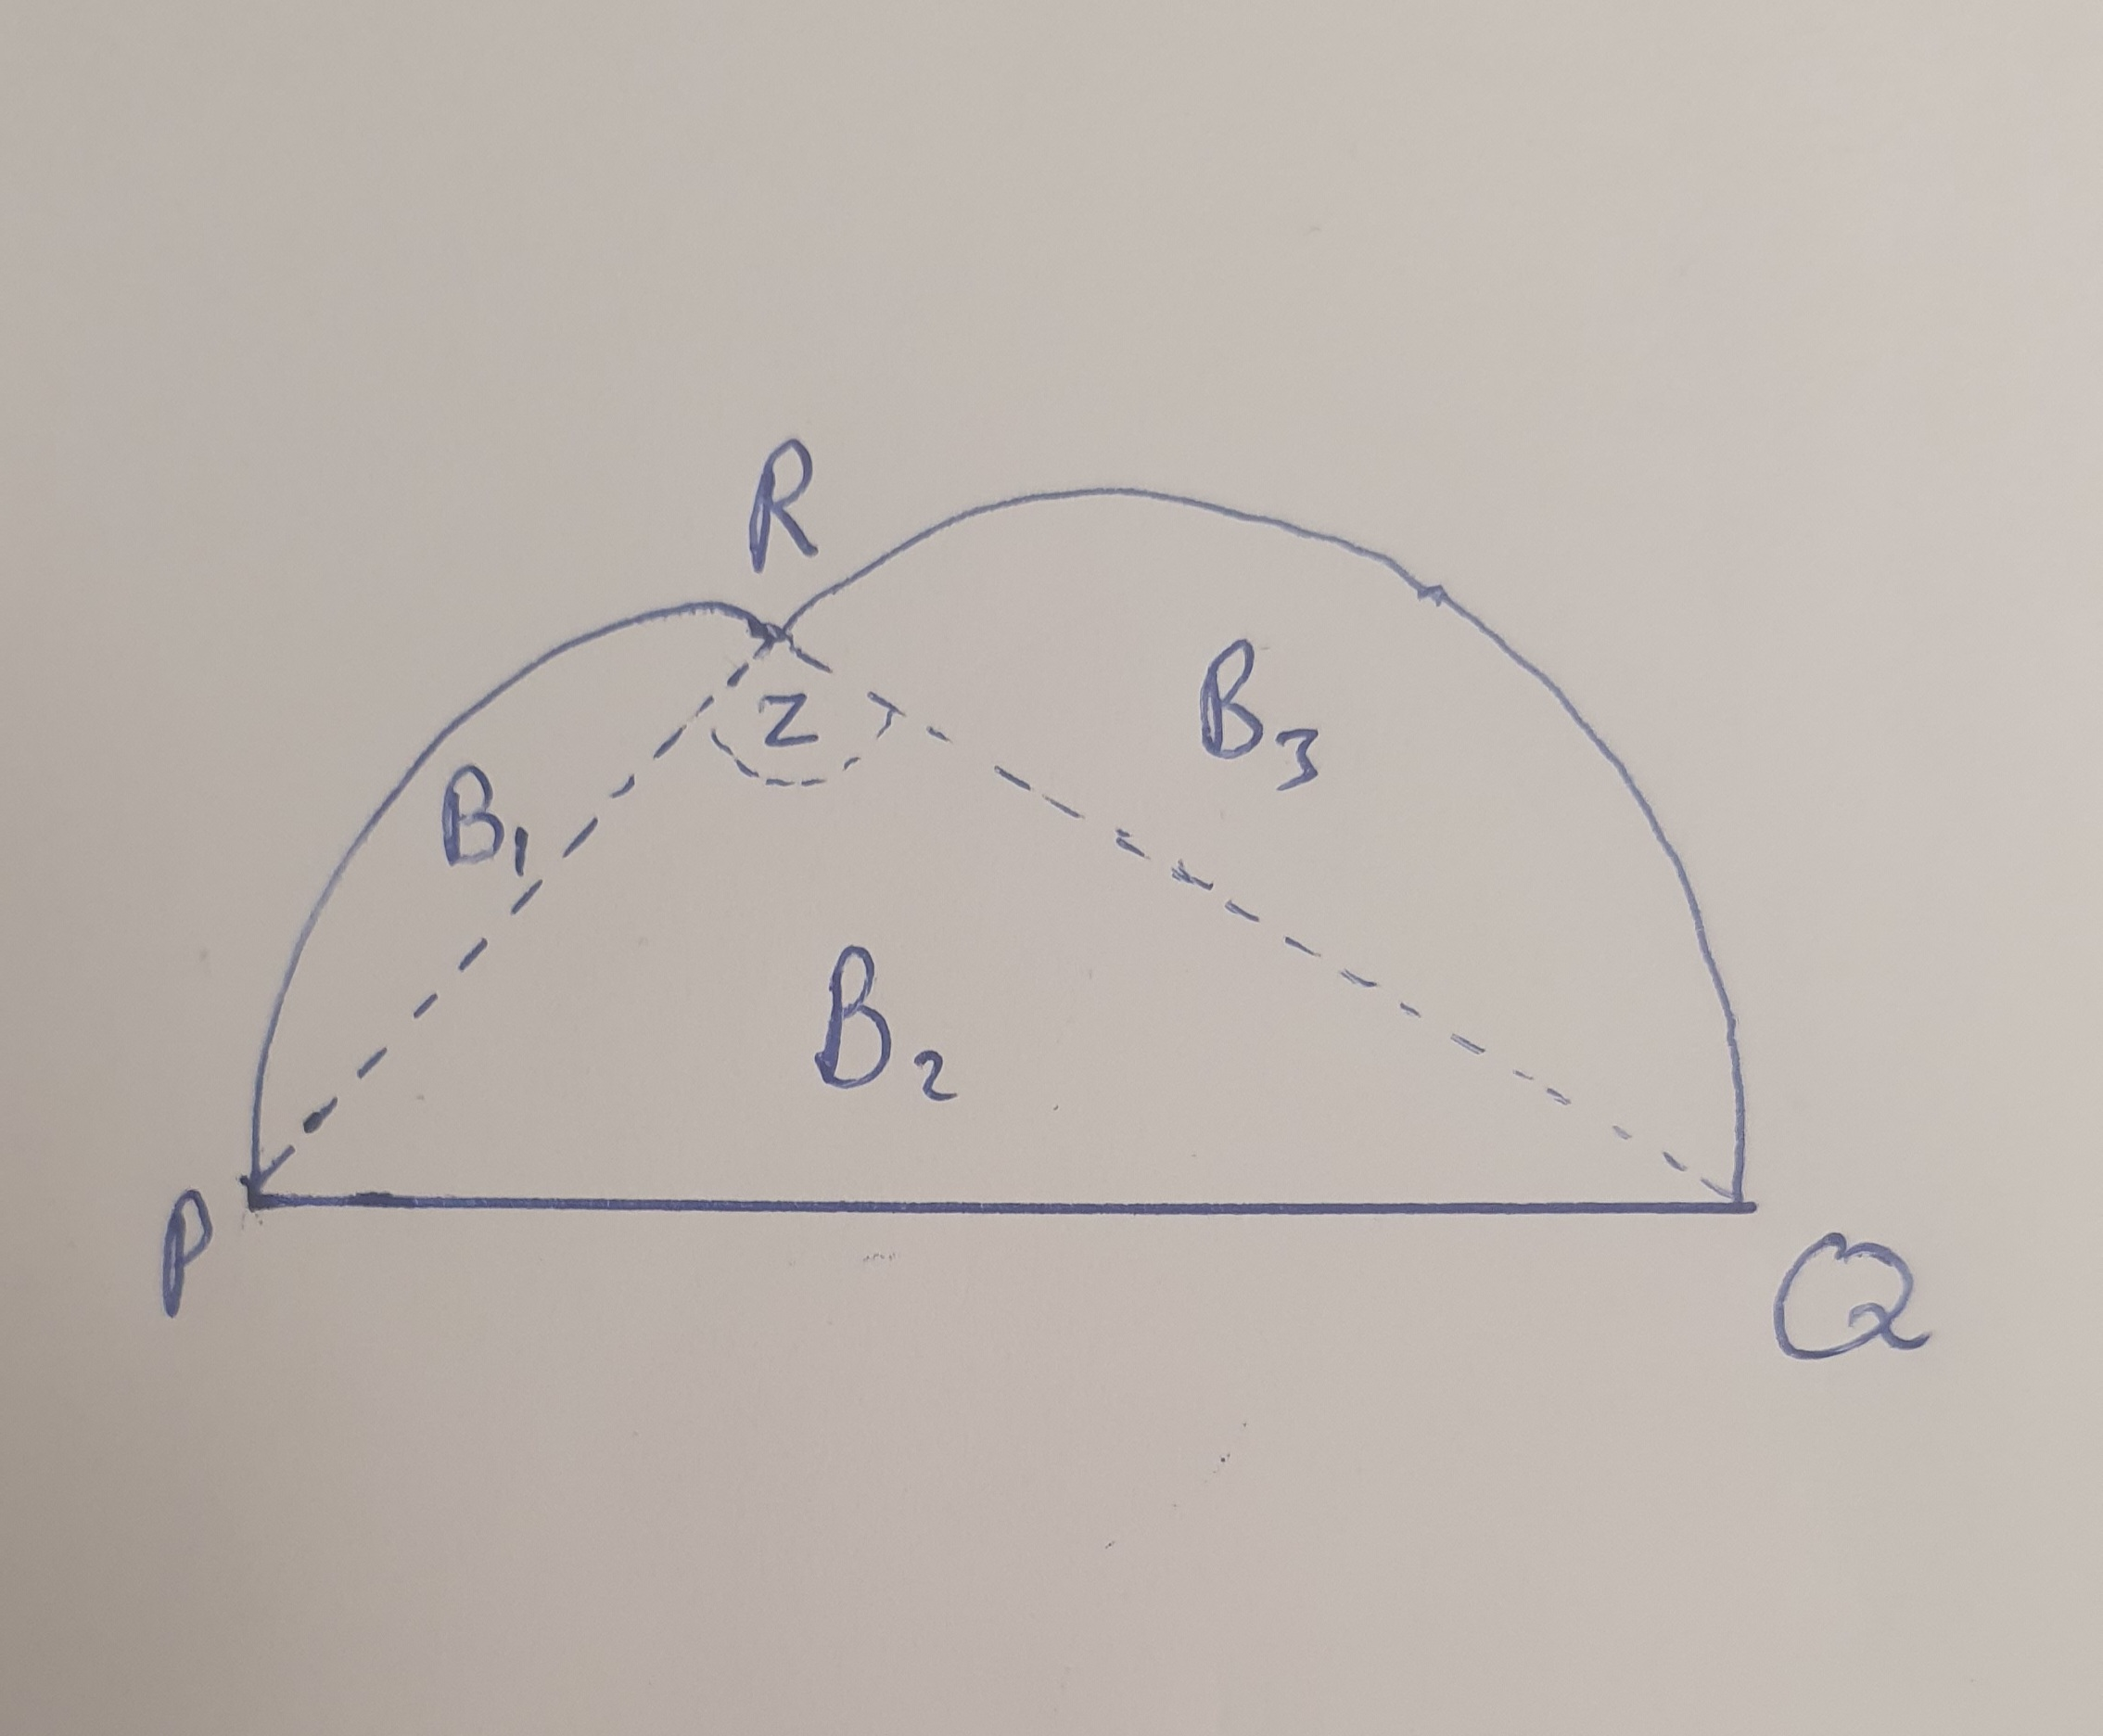
\includegraphics[width=80mm]{isofig4.png}
            \captionof{figure}{Figure VIII}
        \end{minipage}
        \item Next we will need to prove that the region bounded by the line PQ and the arc with length L/2 and endpoints P,Q bounds a region of maximum area and we will prove that the region is a semi-circle. Next we will need to prove that the region bounded by the line PQ and the arc with length L/2 and endpoints P,Q bounds a region of maximum area and we will prove that the region is a semi-circle. for this we are making an assumption which is that of all possible triangles with two sides of given length, the triangle of maximum area is the right triangle with the given sides as the perpendicular sides. This is quite straight forward, consider the figure below.

        \begin{minipage}{\linewidth}
            \centering
            \includegraphics[width=85mm]{isofig3.png}
            \captionof{figure}{Figure IX}
        \end{minipage}
        Well, we know that $g\sin(x)=h$ and the area of triangle, $A=(1/2)fh=(1/2)fg\sin(x)$, clearly A is maximised when x is $90^\circ$ as $\sin(x)$ is then equal to 1.

        Now turning our attention back figure VIII, for the sake of contradiction we will assume that the angle PRQ is not a right angle. Then, we can treat the arc as hinged at R and either open or close it to make the angle at R a right angle, we can do this by adjusting either PR or RQ or maybe both. This adjustment does not alter the arc's length, consequently expanding the total area encapsulated by the arc PRQ and the line PQ. However, this contradicts the maximization achieved by the original arc, which had already optimized the enclosed total area. Therefore, the inscribed angle at R must be a right angle, confirming that the arc is indeed a semi-circle. Now since we have proven that it is a semi circle, we can use this logic and expand it to the whole curve to conclude that it is a circle, by way of reflecting the curve along the original symmetry line.
        
        \item Thus far, we have established that when considering a simple closed curve C with a designated length L, enclosing a region with maximum area, the curve in question must be a circle. Moving forward, we will demonstrate the existence of a maximizer and present this as the comprehensive Isoperimetric problem. In order to achieve this, we will approximate the curve C using a polygonal curve. 
        Use Theorem 7 (we will consider the case where N=2n, as this is just a case of the general theorem)
        Now, let C be a smooth, regular simple closed curve in the plane, with length L and enclosing a region of area A. 
        We can cleverly manipulate our expression from theorem 8 to obtain
	\begin{center}
        $\displaystyle L^{2}\geq4\pi A \frac{\tan(\frac{\pi}{2n})}{\frac{\pi}{2n}}$
	\end{center}
        Now if we carefuly choose our points such that $n \to \infty $,  $L_{n} \to L$ and $A_{n} \to A$, 
        Well, as $n \to \infty$ our expression above becomes
	\begin{center}
        $L^{2}\geq4\pi A$
	\end{center}

        Now we need to show that the equality materialises if and only if the curve in question happens to be a circle. Well if L represents the perimeter of a closed curve, the maximum enclosed area is $\frac{L^{2}}{4\pi}$, conversely if A denotes the area enclosed by a simple closed curve the minimum for the perimeter would be $\sqrt{4 \pi A}$, but the circle is the only curve capable of satisfying such conditions, thus we know that a circle maximises enclosed area among all smooth regular simple closed curves of a fixed length.This confirms the existence of the maximizer. Hence the proof is complete.  
    \end{enumerate}
\end{proof}

\section{E.Schmidt's Proof}
This proof will need:
\begin{enumerate}
	\item AM-GM Inequality 
	\item Cauchy-Schwarz Inequality
	\item $A=\int_{0}^{l} xy' \,dx = -\int_{0}^{l} yx' \,ds$ so $c(s)=(x(s),y(s))$
\end{enumerate}
\textbf{Green's Theorem} $f(x,y)=(u(x,y),v(x,y))$, $\int_{\delta R}\overrightarrow{f} d\overrightarrow{r}$

\begin{proof}
	Let's begin the proof by trying to compute $\iint_{1} 1 \,du\,dv$

	(some figure)

	One condition we know is $\frac{\delta v}{\delta x}-\frac{\delta u}{\delta y}=1$
	
	So we have two solutions:
	\begin{enumerate}
		\item $f(0,x)$
		\item $g(-y,0)$
	\end{enumerate}
	
	taking the line integral of $f(0,x)$ and $g(-y,0)$
	\begin{enumerate}
		\item
			$\int_{C} \overrightarrow{f} \,dr$ \;\;\;where\; $C=(x(t),y(t))$
				
			$= \int_{0}^{l} \overrightarrow{f}(c(t))c'(t) \,dt$ \;\;\;by definition of line integral

			$= \int_{0}^{l} (0,x(t))(x',y') \,dt$
			
			$= \int_{0}^{l} xy' \,dt$ \;\;\;by Green's theorem
		\item
			$\int_{0}^{l} (-y,0)(x',y') \,dt$
			
			$= \int_{0}^{l} x'y \,dt$ \;\;\;by Green's theorem
	\end{enumerate}
	
	(to be finished )
\end{proof}

\chapter{n-Dimensional Case ($\mathbb{R}^n$)}
\section{The Support Function}
The following section introduces the support function, which can be used to ascertain the "height" of a convex body. The support function is a convex function on $\mathbb{R}$ and is compatible with many geometric opetions such as scaling, translation, rotation and importantly the \textbf{Minkowski addition}. These characteristics make the support function one of the most important foundational ideas in convex geometry.

\begin{definition}
	Let $K\subseteq\mathbb{R}^n$ be non-empty, convex and closed. The $support$ $function$ $h(K,\cdot\space)=h_k$ is defined by
	\begin{center}
		$h(K,u):=\sup\{\langle x,u\rangle;x\in K\}$ for $u\in\mathbb{R}^n$
	\end{center}
	Furthermore we define for $u\in dom\,h(K,\cdot)\backslash\{0\}$
	\begin{center}
		$H(K,u):=\{x\in\mathbb{R}^n;\langle x,u\rangle=h(K,u)\}$ a supporting plane of K,
		
		$H^{-}:=\{x\in\mathbb{R}^n;\langle x,u\rangle\leq h(K,u)\}$ a support half space of K, and 
		
		$F(K,u):=H(K,u)\cap K$ a support domain of K
	\end{center}
\end{definition}

\begin{remark}
	The suuport function for $u\in\mathbb{S}^{n-1}\cap dom\,h(K,\cdot)$ can be viewed as the distance of the supporting plane at K with outer unit normal to the origin.(give some figure)
\end{remark}

\begin{remark}
	For $B^{n}$ and $u\in\mathbb{S}^{n-1}$ the support function can be computed easily. For arbirary $x\in B^{n}$ and $u\in\mathbb{S}^{n-1}$ Cauchy Swarz gives us
	\begin{center}
		$|\langle x,u\rangle|\leq||u||\:||x||\leq1$
	\end{center}
	The support function is equal 1 on $B^{n}$ since the maximum is also 1.
\end{remark}

\begin{remark}
	The support funtion has the following properties:
	\begin{enumerate}
		\item $h_{k}\leq h_{L}$ if and only if $K\subseteq L$,
		\item $h(\{z\},u)=\langle x,y\rangle$ for $z,u\in\mathbb{R}^{n}$,
		\item $h(K+t,u)=h(K,u)+\langle t,u\rangle$ for $t,u\in\mathbb{R}^{n}$,
		\item $h(\lambda K, u)=\lambda h(K,u)=h(K,\lambda u)$ for $\lambda\in\mathbb{R}_{0}^{+}$, $u\in\mathbb{R}^{n}$,
		\item $h(-K,u)=h(K,-u)$ for $u\in\mathbb{R}^{n}$,
		\item $h(K,u_{1}+u_{2})\leq h(K,u_{1})+h(K,u_{2})$ for $u_{1},u_{2}\in\mathbb{R}^{n}$,
		\item $h(K,\cdot)=: h_{k}$ is convex.
	\end{enumerate}
\end{remark}

\begin{lemma}
	Let $K,L\in\mathscr{K}^{n}$, then$h(K+L,u)=h(K,u)+h(L,u)$.
\end{lemma}
\begin{proof}
	Let $u\in\mathbb{R}^{n}\backslash\{0\}$.

    First, we show $h(K+L,u)\geq h(K,u)+h(L,u)$. Since $K$ and $L$ are compact, the supremum of the support function is attained. Thus, there exists $x\in K$ and $y\in L$ such that $h(L,u)=\langle y,u\rangle$ and $h(K,u)=\langle x,u\rangle$.

    Then we have
    \begin{center}
        $h(K,u)+h(L,u)=\langle y,u\rangle+\langle x,u\rangle=\langle x+y,u\rangle\leq h(K+L,u)$.
    \end{center}

    Secondly, we want to show $h(K+L,u)\leq h(K,u)+h(L,u)$. Let $z\in K+L$ so that $H(K+L,u)=\langle u,z\rangle$. Then there exists $x\in K$ and $y\in L$ such that $z=x+y$. It follows
    \begin{center}
        $h(K+L,u)=\langle z,u\rangle=\langle x+y,u\rangle=\langle x,u\rangle+\langle y,u\rangle\leq h(K,u)+h(L,u)$.
    \end{center}
    Both inequalities are shown and so the claim follows.
\end{proof}

\section{The Hausdorff Metric}
To prove the continuity of the volume functional and of the support function with respect to convex bodies, we need a metric on the set of convex bodies. This metric will be introduced in the following subsection.

\begin{definition}
    For $K,L\in K^{n}$, define Hausdorff distance or Hausedorff metric by
    \begin{center}
        $\delta(K,L):=\min\{\lambda\geq;K\subseteq L+\lambda B^{n},L\subseteq K+\lambda B^{n}\}$,
    \end{center}
\end{definition}

\begin{remark}
    The Hausdorff distance (Hausdorff metric) on the set of convex bodies. This follows directly from the properties of minima and from the convexity of $K$.
\end{remark}

\begin{lemma}
    Let $K,L\in\mathscr{K}^{n}$, $K,L\subseteq RB^{n}$, where $R>0$, and $u,v\in\mathbb{R}^{n}$. Then
    \begin{center}
        $|h(K,u)-h(L,v)|\leq R|u-v|+\max\{|u|,|v|\}\delta(K,L)$.
    \end{center}
\end{lemma}
\begin{proof}
    Proof can be found in~\cite{schneider2014convex} (section 1.8, Lemma 1.8.12).
\end{proof}

\begin{remark}
    Lemma above proves the local Lipschitz continuity of the support function in both arguments.
\end{remark}

\begin{theorem}
    Let $K,L\in\mathscr{K}^{n}$, then
    \begin{center}
        $\delta(K,L)=\underset{u\in\mathbb{S}^{n-1}}{\sup}|h(K,u)-h(L,u)|=:||\bar{h}_{K}-\bar{h}_{L}||$,
    \end{center}
    where $\displaystyle \bar{h}_{K}=h_{k}|_{\mathbb{S}^{n-1}}$.
\end{theorem}
\begin{proof}
    Let $\delta(K,L)\leq\alpha$. This implies $K\subseteq L+\alpha B^{n}$. For $u\in\mathbb{S}^{n-1}$, it follows 
    \begin{center}
        $h(K,u)\leq h(L+\alpha B^{n},u)=h(L,u)+\alpha h(B^{n},u)=h(L,u)+\alpha$
    \end{center}
    After switching $K$ and $L$, we can conclude for $u\in\mathbb{S}^{n-1}$ that
    \begin{center}
        $|h(K,u)-h(L,u)|\leq\alpha$
    \end{center}
    This implies $||\bar{h}_{K}-\bar{h}_{L}||\leq\delta(K,L)$. Using a similar argument one can show the other estimation.
\end{proof}

\begin{lemma}
    Let $K_{1},K_{2}\in\mathscr{K}^{n}$ and $K_{2}\subseteq\mathring{K}_{1}$. Then there exists $\eta>0$ such that for all $K\in\mathscr{K}^{n}$ with $\delta(K,K_{1})<\eta$, $K_{2}\subseteq K$ holds.
\end{lemma}
\begin{proof}
    Can be found in~\cite{schneider2014convex} (Section 1.8, Lemma 1.8.18)
\end{proof}
    
\section{Volume and Surface Measure}
In this subsection, we will introduce the volume functional and show its continuity. The results of this subsection are important in the proof of Brunn-Minkowski.

\begin{definition}
	Let $M\subseteq\mathbb{R}^{n}, p\geq0$. For $\delta>0$ define
	\begin{center}
		$\displaystyle \mathscr{H}_{\delta}^{P}(M):=\inf\{\sum\limits_{i=1}^{\infty}\alpha(p)(\frac{diam C_{i}}{2})^{p};(C_{i})_{i\in\mathbb{N}}$ open sets in $\mathbb{R}^n$

		\hspace{1cm}with $diam C_{i}\leq\delta$ and $M\subseteq\underset{i\in\mathbb{N}}{\cup}{C_{i}}\}$
	\end{center}
	with $\alpha(p)=\frac{\pi^{\frac{p}{2}}}{\Gamma(p)(\frac{p}{2}+1)}$ for $p\neq0$, where $\Gamma(p):=\int_{0}^{\infty}t^{-1}e^{-t}\,dt$ and $\alpha(0)=0$.
	
	Define the p-dimensional Hausdorff measure of $M$ by
	\begin{center}
		$\mathscr{H}^{p}(M):=\underset{\delta>0}{\sup}\mathscr{H}_{\delta}^{p}(M)=\underset{\delta\to0}{\lim}\mathscr{H}_{\delta}^{p}(M)$.
	\end{center}
\end{definition}

\begin{remark}
	Let $t\in\mathbb{R}^{n}$ and $\lambda\in\mathbb{R}$, then we have
	\begin{center}
		$\mathscr{H}^{p}(\lambda M)=\lambda^{p}\mathscr{H}^{p}(M)$ and $\mathscr{H}^{p}(M=t)=\mathscr{H}^{p}(M)$.
	\end{center}
	Furthermroe, for $A\subseteq B$ we have $\mathscr{H}^{p}(A)\leq\mathscr{H}^{p}(B)$.
\end{remark}

\begin{definition}
	The volume funcational $V_{n}$ on $\mathscr{K}^{n}$ is defined by the restriction of the $n$-dimensional Hausdorff measure on $\mathscr{K}^{n}$.
\end{definition}

\begin{theorem}
	The volume functional $V_{n}:\mathscr{K}^{n}\to\mathbb{R}$ is continuous.
\end{theorem}
\begin{proof}
    \textbf{Case 1 $\mathrm{V}_{n}(\mathrm{K})=0$:}
    Let $\overline{a}\in\mathscr{K}^{n}$ and, without loss of generality, assume $\delta(K,\overline{K})=\alpha\leq1$. Thus, it holds that $\overline{K}\subseteq K+\alpha B^{n}$. Since $V_{0}(K)=0$ and $K$ is convex, we know that $K$ has to be contained in a hyperplane. From the monotony of the Hausdorff measure it follows for $u$ orthogonal on the hyperplane, that
    \begin{center}
        $V_{n}(\mathrm{K})\leq \mathrm{V}_{n}(K+\alpha \mathrm{B}_{n})$

        $=\int_{-\alpha}^{\alpha}\mathrm{V}_{n-1}([\mathrm{K}+\alpha \mathrm{B}^{n}]\cap\mathrm{H}_{u,\zeta})\,d\zeta$

        $\leq\int_{-\alpha}^{\alpha}\mathrm{V}_{n-1}(K+(\alpha\mathrm{B}^{n}\cap\mathrm{H}_{u,\zeta}))\,d\zeta$

        $=2\alpha \mathrm{V}_{n-1}(K+(\alpha\mathrm{B}^{n}\cap\mathrm{H}_{u,0}))$

        $\overset{\alpha\leq1}{\leq}\underbrace{2\mathrm{~V}_{n-1}\left(\mathrm{~K}+\left(\mathrm{B}^n\cap \mathrm{H}_{u, 0}\right)\right)}_{:=c(\mathrm{~K})}\cdot\alpha$,
    \end{center}
    In the second line we used that $K+\alpha B^{n}$ varies in the fixed coordinate of $K$ by $2\alpha$. Since $c(K)$ is fixed and does not depend on $\alpha$ the continuity follows.

    \textbf{Case 2 $\mathrm{V}_{n}(\mathrm{K})>0$:}
    Without loss of generality, assume that $0\in\overset{\circ}{\mathrm{K}}$ (if not, we can shift it, since the Hausdorff measure is invariant under shifts). Let $\epsilon>0$ and choose $\lambda>1$ such that
    \begin{center}
        $(\lambda^{n}-1)\lambda^{n}\mathrm{V}_{n}(\mathrm{K})<\epsilon$
    \end{center}
    and $\rho>0$ so that $\rho\mathrm{B}^{n}\subseteq\overset{\circ}{\mathrm{K}}$. From Lemma 13, we 
    know that there is an $\alpha>0$ with $\alpha\leq(\lambda-1)\rho$ so that $\rho\mathrm{B}_{n}\subseteq\overset{\circ}{\mathrm{K}}\subseteq\overline{\mathrm{K}}$. For all $\mathrm{K}$ with $\delta(K,\overline{\mathrm{K}})<\alpha$. From $\delta(\mathrm{K},\overline{\mathrm{K}})<\alpha$ it follows
    \begin{center}
        $\mathrm{K}\subseteq\overline{\mathrm{K}}+\alpha\mathrm{B}^{n}\subseteq\overline{\mathrm{K}}+(\lambda-1)\rho\mathrm{B}^{n}\subseteq\overline{\mathrm{K}}+(\lambda-1)\overline{\mathrm{K}}=\lambda\overline{\mathrm{K}}$
    \end{center}
    With the same argument, we can also show that $\overline{\mathrm{K}}\subseteq\lambda\mathrm{K}$. Hence we have the inequalities $\mathrm{V}_{n}(\mathrm{K})\leq\mathrm{V}_{n}(\lambda\mathrm{K})=\lambda^{n}\mathrm{V}_{n}(\overline{\mathrm{K}})$ and $\mathrm{V}(\overline{\mathrm{K}})\leq\mathrm{V}_{n}(\lambda\mathrm{K})=\lambda^{n}\mathrm{V}_{n}{\mathrm{K}}$. \newline
    This implies
    \begin{center}
        $\mathrm{V}_{n}(\mathrm{K})-\mathrm{V}_{n}(\overline{\mathrm{K}})\leq(\lambda^{n}-1)\mathrm{V}_{n}(\overline{\mathrm{K}})\leq(\lambda^{n}-1)\lambda^{n}\mathrm{V}_{n}(\mathrm{K})$ and

        $\mathrm{V}_{n}(\overline{\mathrm{K}})-\mathrm{V}_{n}(\mathrm{K})\leq(\lambda^{n}-1)\mathrm{V}_{n}(\mathrm{K})\overset{\lambda>1}{\leq}(\lambda^{n}-1)\lambda^{n}\mathrm{V}_{n}(\mathrm{K})$.
    \end{center}
    As a consequence we have the estimate
    \begin{center}
        $|\mathrm{V}_{n}(\mathrm{K})-\mathrm{V}_{n}(\overline{\mathrm{K}})|\leq(\lambda^{n}-1)\lambda^{n}\mathrm{V}_{n}(\mathrm{K})<\epsilon$.
    \end{center}
    This implies the continuity of $\mathrm{V}_{n}$.
\end{proof}

\begin{theorem}(Steiner's Formula)
    There are $\mathrm{V}_{m}:\mathscr{K}^{n}\to\mathbb{R}$ and cofficients $k_i\in\mathbb{R}$ for $i=0,1,\dots,n$ such that 
    \begin{center}
        $\mathrm{V}_{n}(\mathrm{K}+\rho\mathrm{B}^{n})=\overset{n}{\underset{m=0}{\sum}}\rho^{n-m}k_{n-m}\mathrm{V}_{m}(\mathrm{K})$
    \end{center}
    for all $\mathrm{K}\in\mathscr{K}^{n}$, $\rho\geq0$.
\end{theorem}
A proof of this can be found in~\cite{schneider2014convex} (Theorem 4.2.1).

\begin{remark}
    Steiner’s formula implies that $\rho\mapsto\mathrm{V}_{n}(\mathrm{K}+\rho\mathrm{B}^{n})$ is a polynomial of degree $n$.
\end{remark}

\begin{definition} (Surface Measure)
    Let $\mathrm{K}\subseteq\mathscr{K}^{n}$. Then we define the \textit{surface measure} of $\mathrm{K}$ by
    \begin{center}
        $\mathrm{S}(\mathrm{K}):=\underset{\rho\to0}{\lim}\frac{\mathrm{V}_{n}(\mathrm{K}+\epsilon\mathrm{B}^{n})-\mathrm{V}_{n}(\mathrm{K})}{\rho}$.
    \end{center}
\end{definition}

\begin{remark}
    This limit exists, because $\mathrm{V}_{n}(\mathrm{K}+\epsilon\mathrm{B}^{n})$ is a polynomial and, therefore, it is smooth.
\end{remark}

\begin{remark}
    Let $\mathrm{B}^{n}\subseteq\mathbb{R}^{n}$ be a ball. We then have
    \begin{center}
        $\mathrm{S}(r\mathrm{B}^{n})=nr^{n-1}\mathrm{V}_{n}(\mathrm{B}^{n})$
    \end{center}
\end{remark}
\begin{proof}
    Using the convexivity of $\mathrm{B}^{n}$ and the properties of the volume functional, we can compute
    \begin{center}
        $\displaystyle \mathrm{S}(\mathrm{B}^{n})=\underset{\rho\downarrow0}{\lim}\frac{\mathrm{V}_{n}(\mathrm{K}+\epsilon\mathrm{B}^{n})-\mathrm{V}_{n}(\mathrm{K})}{\rho}$

        $\displaystyle =\underset{\rho\downarrow0}{\lim}\frac{((r+\rho)^{n}-r^{n})\mathrm{V}_{n}(\mathrm{B}^{n})}{\epsilon}$

        $\displaystyle =\mathrm{V}_{n}(\mathrm{B}^{n})\underset{\rho\downarrow0}{\lim}\frac{(r+\rho)^{n}-r^{n}}{\epsilon}=\mathrm{V}_{n}(\mathrm{B})\cdot n\cdot r^{n−1}$.
    \end{center}
\end{proof}

\section{Brunn-Minkowski Theorem}
\section{3-Dimensional Case ($\mathbb{R}^3$)}
\subsection{Proof of 3-Dimensional Case}
\section{Proof of the Isoperimetric Inequality in n-Dimension}

\chapter{Manifolds}

\bibliography{The-Isoperimetric-Problem-References}
\bibliographystyle{unsrt}
\end{document}